\def\year{2022}\relax
%File: formatting-instructions-latex-2022.tex
%release 2022.1
\documentclass[letterpaper]{article} % DO NOT CHANGE THIS
\usepackage{aaai22}  % DO NOT CHANGE THIS
\usepackage{times}  % DO NOT CHANGE THIS
\usepackage{helvet}  % DO NOT CHANGE THIS
\usepackage{courier}  % DO NOT CHANGE THIS
\usepackage{hyperref}
\usepackage[hyphens]{url}  % DO NOT CHANGE THIS
\usepackage{graphicx} % DO NOT CHANGE THIS
\urlstyle{rm} % DO NOT CHANGE THIS
\def\UrlFont{\rm}  % DO NOT CHANGE THIS
\usepackage{natbib}  % DO NOT CHANGE THIS AND DO NOT ADD ANY OPTIONS TO IT
\usepackage{caption} % DO NOT CHANGE THIS AND DO NOT ADD ANY OPTIONS TO IT
\DeclareCaptionStyle{ruled}{labelfont=normalfont,labelsep=colon,strut=off} % DO NOT CHANGE THIS
\frenchspacing  % DO NOT CHANGE THIS
\setlength{\pdfpagewidth}{8.5in}  % DO NOT CHANGE THIS
\setlength{\pdfpageheight}{11in}  % DO NOT CHANGE THIS
%
% These are recommended to typeset algorithms but not required. See the subsubsection on algorithms. Remove them if you don't have algorithms in your paper.
\usepackage{algorithm}
\usepackage{algorithmic}
\usepackage{amsmath,epsfig}

%
% These are are recommended to typeset listings but not required. See the subsubsection on listing. Remove this block if you don't have listings in your paper.
\usepackage{newfloat}
\usepackage{listings}
\lstset{%
	basicstyle={\footnotesize\ttfamily},% footnotesize acceptable for monospace
	numbers=left,numberstyle=\footnotesize,xleftmargin=2em,% show line numbers, remove this entire line if you don't want the numbers.
	aboveskip=0pt,belowskip=0pt,%
	showstringspaces=false,tabsize=2,breaklines=true}
\floatstyle{ruled}
\newfloat{listing}{tb}{lst}{}
\floatname{listing}{Listing}
%
%\nocopyright
%
% PDF Info Is REQUIRED.
% For /Title, write your title in Mixed Case.
% Don't use accents or commands. Retain the parentheses.
% For /Author, add all authors within the parentheses,
% separated by commas. No accents, special characters
% or commands are allowed.
% Keep the /TemplateVersion tag as is
\pdfinfo{
/Title (Modified ResNet-18)
/Author (AAAI Press Staff, Pater Patel Schneider, Sunil Issar, J. Scott Penberthy, George Ferguson, Hans Guesgen, Francisco Cruz, Marc Pujol-Gonzalez)
/TemplateVersion (2022.1)
}

% DISALLOWED PACKAGES
% \usepackage{authblk} -- This package is specifically forbidden
% \usepackage{balance} -- This package is specifically forbidden
% \usepackage{color (if used in text)
% \usepackage{CJK} -- This package is specifically forbidden
% \usepackage{float} -- This package is specifically forbidden
% \usepackage{flushend} -- This package is specifically forbidden
% \usepackage{fontenc} -- This package is specifically forbidden
% \usepackage{fullpage} -- This package is specifically forbidden
% \usepackage{geometry} -- This package is specifically forbidden
% \usepackage{grffile} -- This package is specifically forbidden
% \usepackage{hyperref} -- This package is specifically forbidden
% \usepackage{navigator} -- This package is specifically forbidden
% (or any other package that embeds links such as navigator or hyperref)
% \indentfirst} -- This package is specifically forbidden
% \layout} -- This package is specifically forbidden
% \multicol} -- This package is specifically forbidden
% \nameref} -- This package is specifically forbidden
% \usepackage{savetrees} -- This package is specifically forbidden
% \usepackage{setspace} -- This package is specifically forbidden
% \usepackage{stfloats} -- This package is specifically forbidden
% \usepackage{tabu} -- This package is specifically forbidden
% \usepackage{titlesec} -- This package is specifically forbidden
% \usepackage{tocbibind} -- This package is specifically forbidden
% \usepackage{ulem} -- This package is specifically forbidden
% \usepackage{wrapfig} -- This package is specifically forbidden
% DISALLOWED COMMANDS
% \nocopyright -- Your paper will not be published if you use this command
% \addtolength -- This command may not be used
% \balance -- This command may not be used
% \baselinestretch -- Your paper will not be published if you use this command
% \clearpage -- No page breaks of any kind may be used for the final version of your paper
% \columnsep -- This command may not be used
% \newpage -- No page breaks of any kind may be used for the final version of your paper
% \pagebreak -- No page breaks of any kind may be used for the final version of your paperr
% \pagestyle -- This command may not be used
% \tiny -- This is not an acceptable font size.
% \vspace{- -- No negative value may be used in proximity of a caption, figure, table, section, subsection, subsubsection, or reference
% \vskip{- -- No negative value may be used to alter spacing above or below a caption, figure, table, section, subsection, subsubsection, or reference

\setcounter{secnumdepth}{0} %May be changed to 1 or 2 if section numbers are desired.

% The file aaai22.sty is the style file for AAAI Press
% proceedings, working notes, and technical reports.
%

% Title

% Your title must be in mixed case, not sentence case.
% That means all verbs (including short verbs like be, is, using,and go),
% nouns, adverbs, adjectives should be capitalized, including both words in hyphenated terms, while
% articles, conjunctions, and prepositions are lower case unless they
% directly follow a colon or long dash
\title{PokeGAN \\ Generating New Pokemon Using Generative Adversarial Networks}
\author{
    %Authors
    % All authors must be in the same font size and format.
    Parisima Abdali , \textsuperscript{}
    Karan Vora \textsuperscript{}
}
\affiliations{ New York University \\ pa2297@nyu.edu, kv5124@nyu.edu \\
\href{https://github.com/parisimaa/PokGAN}
{\underline{github.com/PokGAN}}

}

%Example, Single Author, ->> remove \iffalse,\fi and place them surrounding AAAI title to use it
\iffalse
\title{My Publication Title --- Single Author}
\author {
    Author Name
}
\affiliations{
    Affiliation\\
    Affiliation Line 2\\
    name@example.com
}
\fi

\iffalse
%Example, Multiple Authors, ->> remove \iffalse,\fi and place them surrounding AAAI title to use it
\title{My Publication Title --- Multiple Authors}
\author {
    % Authors
    First Author Name,\textsuperscript{\rm 1}
    Second Author Name, \textsuperscript{\rm 2}
    Third Author Name \textsuperscript{\rm 1}
}
\affiliations {
    % Affiliations
    \textsuperscript{\rm 1} Affiliation 1\\
    \textsuperscript{\rm 2} Affiliation 2\\
    firstAuthor@affiliation1.com, secondAuthor@affilation2.com, thirdAuthor@affiliation1.com
}
\fi


% REMOVE THIS: bibentry
% This is only needed to show inline citations in the guidelines document. You should not need it and can safely delete it.
\usepackage{bibentry}
% END REMOVE bibentry

\begin{document}

\maketitle

\begin{abstract}
In our project, we utilized Generative Adversarial Networks (GANs)\cite{GAN} to analyze a custom Pokémon dataset consisting of more than 1000 unique Pokémon images. The main goal was to harness the potential of GANs for generating novel Pokémon spirits. However, GANs often face challenges regarding stability during training, which can result in lower quality outputs. To overcome this limitation, we explored the application of Autoencoding Generative Adversarial Networks (AEGANs)\cite{AEGAN} and evaluated their performance against traditional GANs to achieve higher quality results.
\end{abstract}

\section{Introduction}
Generative models via adversarial process (GANs) \cite{GAN} are a class of machine learning models that are widely used in the field of artificial intelligence and specifically in the domain of generative modeling.

Our objective is to develop a GAN-based system capable of generating novel and visually compelling Pokémon spirits that align with the patterns and aesthetics found in the provided dataset. The GAN architecture consists of a generator and a discriminator to learn the patterns, characteristics, and visual qualities exhibited by Pokémon in the custom dataset with over 1000 images. \\
The problem involves the following key challenges: \\
1) Developing a GAN architecture that can effectively capture the intricate patterns, shapes, colors, and unique characteristics exhibited by Pokémon spirits from the provided dataset. \\
2) Training the generator network to produce synthetic Pokémon images that closely resemble real Pokémon spirits, ensuring a high level of visual fidelity and realism. \\
3) Training the discriminator network to accurately distinguish between real Pokémon images from the dataset and synthetic images generated by the generator, thereby improving the overall quality of the generated Pokémon spirits. \\
4) Ensuring that the GAN architecture can generate a diverse range of new Pokémon spirits that go beyond simple replication of existing examples, and expanding the design space for Pokémon characters. 
\begin{figure}[htbp]
\captionsetup[subfigure]{justification=centering}
  \centering
  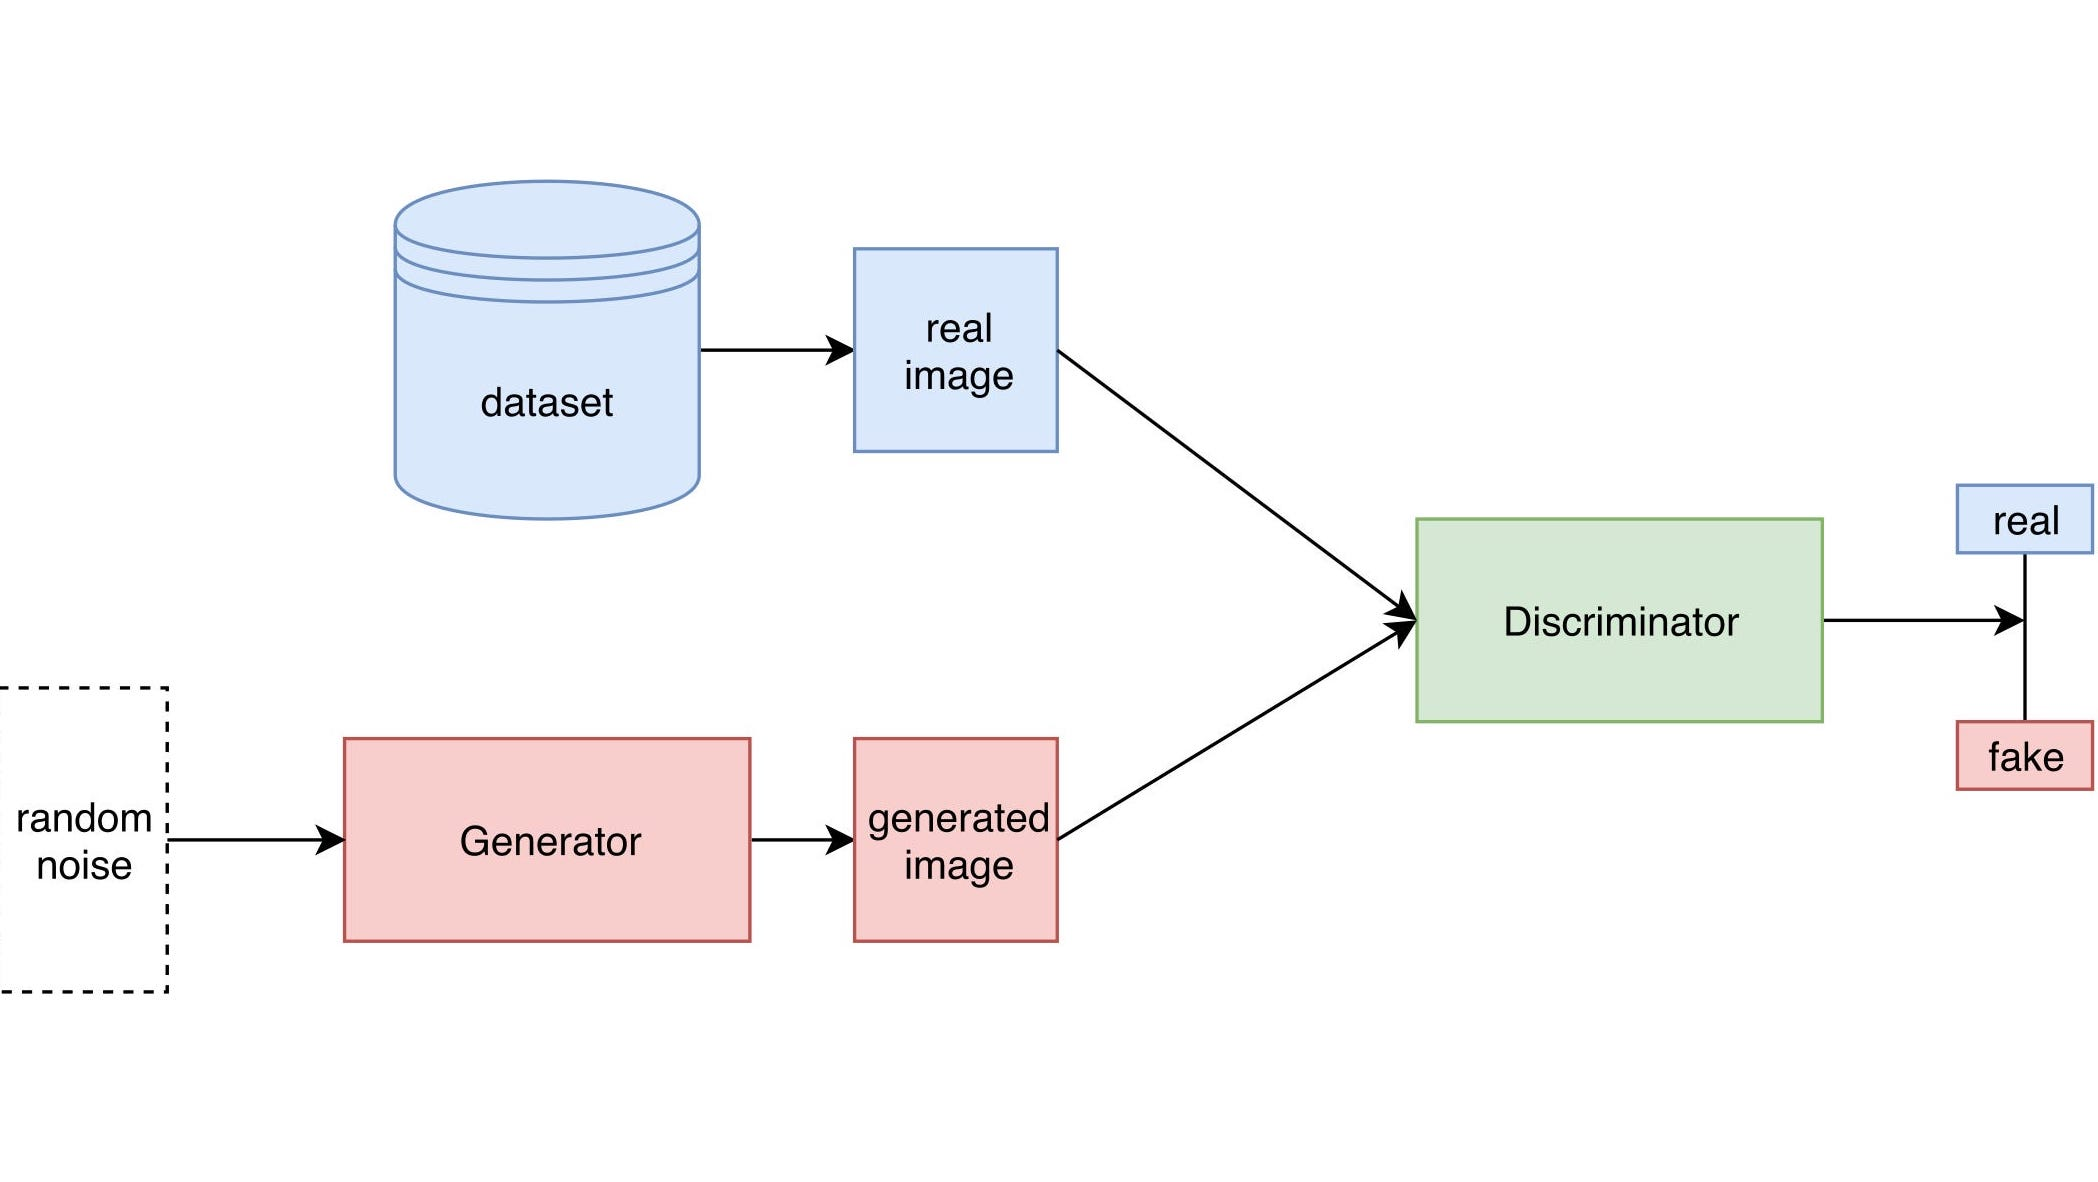
\includegraphics[scale = 0.12]{image/GAN.jpg}
  \caption{GAN network}\label{fig:GAN net}
%  \label{fig:fig2}
\end{figure}

\begin{figure}[htbp]
\captionsetup[subfigure]{justification=centering}
  \centering
  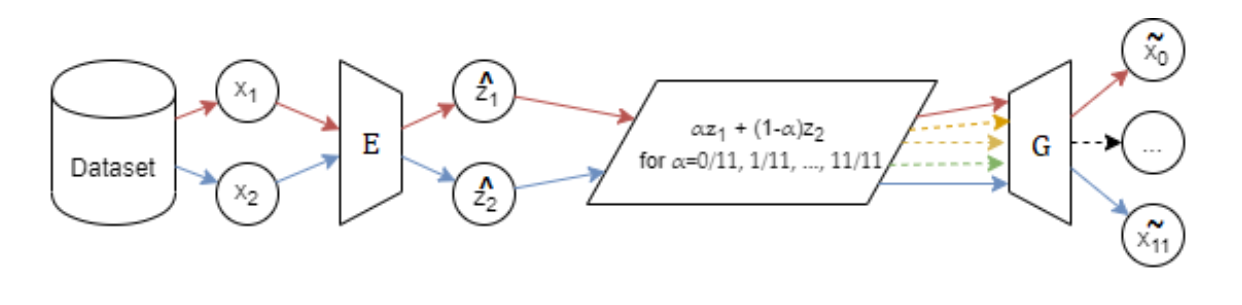
\includegraphics[scale = 0.33]{image/AEGAN.png}
  \caption{AEGAN network}\label{fig:AEGAN net}
%  \label{fig:fig2}
\end{figure}

Although GANs are renowned for their ability to generate synthetic images, their training process can be unstable, potentially affecting the quality of generated shapes. In our project, we explored an alternative model known as the Autoencoding Generative Adversarial Network (AEGAN)\cite{AEGAN}. This four-network model learns a bijective mapping between a defined latent space and a specified sample space by employing adversarial and reconstruction losses for both the generated images and latent vectors. Our aim is to compare the performance of AEGAN with traditional GANs.

\begin{figure*}[htbp]
\captionsetup[subfigure]{justification=centering}
  \centering
  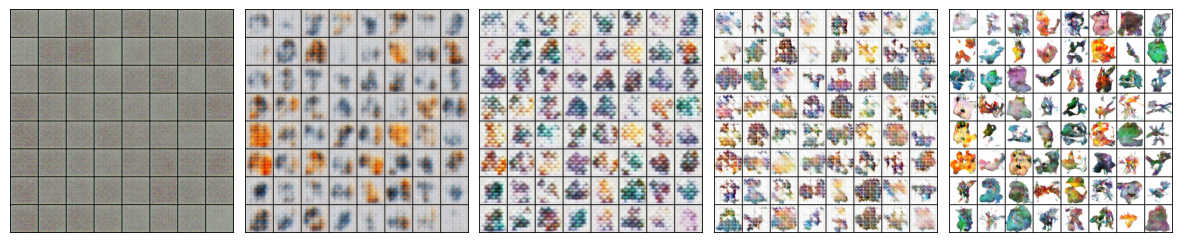
\includegraphics[scale = 0.55]{image/process.png}
  \caption{Process of generating new Pokémons for different epochs using GAN model}\label{fig:pok1}
%  \label{fig:fig2}
\end{figure*}
\begin{figure*}[htbp]
\captionsetup[subfigure]{justification=centering}
  \centering
  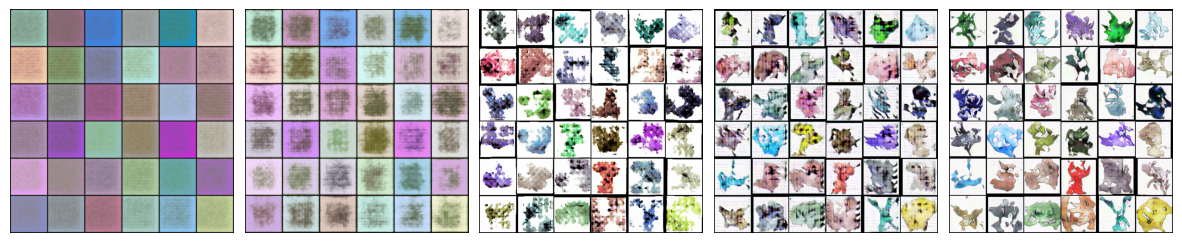
\includegraphics[scale = 0.55]{image/AEGAN process.png}
  \caption{Process of generating new Pokémons for different epochs using AEGAN model}\label{fig:pok2}
%  \label{fig:fig2}
\end{figure*}
 
\section{Model Background}

The fundamental idea behind GANs is to train two neural networks, known as the generator and the discriminator, in a competitive setting. The generator network learns to generate synthetic data, such as Pokémon images in our case, by producing samples that are difficult to distinguish from real data. On the other hand, the discriminator network learns to classify between real and fake data, aiming to correctly identify the synthetic samples generated by the generator. \\
D and G play the following two-player minimax game with value function V (G, D)\cite{GAN}:

\begin{gather}\label{eq:1}
    \begin{aligned}
        \min_{G}\max_{D} V(D,G) = E_{x \sim p_{data}(x)}|log D(x)| +  \\ E_{z \sim p_{z}(z)}|log (1 - D(G(z)))|
    \end{aligned}
\end{gather}

Where,
\(D(\mathbf{x})\) represents the output of the discriminator network for a real input sample \(\mathbf{x}\).
\(G(\mathbf{z})\) represents the output of the generator network for a random noise input \(\mathbf{z}\).
\(p_{\text{data}}(\mathbf{x})\) represents the distribution of real data samples.
\(p_{\mathbf{z}}(\mathbf{z})\) represents the distribution of random noise input.
\(\mathbb{E}\) represents the expectation operator. \\
In the discriminator play, the goal is to minimize the discriminator's loss by correctly classifying real data samples (\(D(\mathbf{x})\)) as real and generated samples (\(D(G(\mathbf{z}))\)) as fake. \\
In the generator play, the goal is to minimize the generator's loss by generating samples (\(G(\mathbf{z})\)) that are classified as real (\(D(G(\mathbf{z}))\)) by the discriminator.

Similarly, the Autoencoding Generative Adversarial Network (AEGAN) extends the GAN framework by incorporating an encoder component. However, instead of directly using a formula like Equation \ref{eq:1}, AEGANs employ a combination of adversarial loss and reconstruction loss to train the networks.

The adversarial loss has four components: we consider generated samples $G(z) = \hat{x}$, encoded samples $E(x) = \hat{z}$, autoencoded samples $G(E(x)) = \widetilde{x}$, and autoencoded latent vectors $E(G(z)) = \widetilde{z}$, where $x$ are real samples drawn from the dataset and $z$ are latent vectors drawn randomly from some distribution. Thus, the four components to the adversarial loss are:

\begin{gather}\label{eq:2}
    \begin{aligned}
        {L}_{GAN_{\hat{x}}}(G, D_x) =E_{x \sim p_{data}}[\log D_{x}(x)] + \\E_{z \sim p(z)}[\log (1 - D_{x}(G(z))]
    \end{aligned}
\end{gather}
\begin{gather}\label{eq:3}
    \begin{aligned}
        {L}_{GAN_{\tilde{x}}}(G, E, D_x) = E_{x \sim p_{data}}[\log D_{x}(x)] + \\E_{x \sim p_{data}}[\log (1 - D_{x}(G(E(x)))]
    \end{aligned}
\end{gather}
\begin{gather}\label{eq:4}
    \begin{aligned}
        {L}_{GAN_{\hat{z}}}(E, D_z) = E_{x \sim p(z)}[\log D_{z}(z)] + \\E_{z \sim p_{data}}[\log (1 - D_{z}(E(x))]
    \end{aligned}
\end{gather}
\begin{gather}\label{eq:5}
    \begin{aligned}
        {L}_{GAN_{\tilde{z}}}(G, E, D_z) = E_{x \sim p(z)}[\log D_{z}(z)] +\\ E_{x \sim p(z)}[\log (1 - D_{z}(E(G(z)))]
    \end{aligned}
\end{gather}

Which, summed, form the adversarial loss ${L}_{GAN}(G, E, D_x, D_z)$\cite{AEGAN}. 

Because the goal is to learn a bijective mapping, it is important that $E$ undoes $G$ and vice-versa. Thus, a reconstruction loss is used:
\begin{gather}\label{eq:6}
    \begin{aligned}
      {L}_{r}(G, E) = \lambda_{rx}E_{x \sim p_{data}}[\left| \left| G(E(x)) - x \right| \right|_1] +\\ \lambda_{rz}E_{z \sim p(z)}[\left| \left| E(G(z)) - z \right| \right|_2] 
    \end{aligned}
\end{gather}
Where $\lambda_{rx}$ and $\lambda_{rz}$ are hyperparamters for controlling the weight of the sample reconstruction and latent vector reconstruction, respectively. The $L_1$ loss is used for sample reconstruction because it is known to result in less bluriness than $L_2$ in image reconstruction \cite{AEGAN}.

The full AEGAN objective is thus:
\begin{gather}\label{eq:7}
    \begin{aligned}
     {L}_{AEGAN}(G, E, D_x, D_z) = \\ {L}_{GAN}(G, E, D_x, D_z) + {L}_{r}(G, E) 
    \end{aligned}
\end{gather}


% \begin{figure}[htbp]
% \captionsetup[subfigure]{justification=centering}
%   \centering
%   \includegraphics[scale = 0.5]{image/resnet-block.png}
%   \caption{ResNet Block}
% %  \label{fig:fig2}
% \end{figure}

\section{Network Architecture}
\subsection{1) GAN (Generative Adversarial Network):}

The basic block of a GAN consists of two main components: a generator and a discriminator.

Generator: The generator takes a random input, often referred to as a latent vector or noise, and generates synthetic data, such as images, based on that input. The generator aims to generate data that resembles the real data from the training set.

Discriminator: The discriminator acts as a classifier that tries to distinguish between real data from the training set and synthetic data generated by the generator. It receives both real and synthetic data as input and outputs a probability score, indicating the likelihood of the input being real or fake.

During training, the generator and discriminator are trained simultaneously in an adversarial manner. The generator aims to produce synthetic data that the discriminator cannot distinguish from real data, while the discriminator tries to improve its ability to accurately classify real and fake data. This adversarial process drives the models to improve over time.
\subsection{2) AEGAN (Autoencoding Generative Adversarial Network):}
The AEGAN is an extension of the GAN architecture that incorporates an additional component called the encoder or autoencoder\cite{encod}.

Encoder: The encoder takes a real or synthetic input data and maps it to a lower-dimensional latent space. This latent representation aims to capture the essential features and characteristics of the input data.

The AEGAN architecture typically consists of four main components: encoder, generator, discriminator, and reconstruction loss.

During training, the generator aims to produce synthetic data that looks realistic and aligns with the patterns in the training set. The discriminator tries to accurately classify between real and synthetic data. Additionally, a reconstruction loss is introduced, which compares the original input data with the data reconstructed from the latent space by the encoder and generator. This loss encourages the generator and encoder to preserve the information and characteristics of the input data throughout the encoding-decoding process.
\subsubsection{Optimizer}
The optimizer used in the code is Adam optimizer \cite{adam}. It is a popular optimization algorithm commonly used in deep learning. Adam stands for Adaptive Moment Estimation, and it combines the concepts of gradient descent with momentum and RMSprop (optimizer for both GAN and AEGAN is the same). 

In our model, both the generator and discriminator are optimized using the Adam optimizer. The generator and discriminator models are wrapped in the $torch.nn.DataParallel$ module to enable parallel training across multiple GPUs.
\subsubsection{Hyper-parameters}
These hyperparameters govern various aspects of the training process, including the batch size, image size, learning rate, and number of training epochs, all of which can influence the model's performance and training speed. In our implementation, we selected a batch size of 128 and trained the model for 500 epochs in GAN network and for AEGAN we have 32 for batch size. Please note that due to system limitations and scheduling constraints, we were only able to train for a limited number of epochs, as depicted in the graph (same number of epochs have been used for both GAN and AEGAN).

Furthermore, we set the learning rate to 0.00028 for both the generator and discriminator models. The $betas$ parameter consists of a tuple with two values, which are employed to calculate the running averages of the gradient and its square. In our model, we configured the betas values as (0.5, 0.999) for both the generator and discriminator. In AEGAN case we used learning rate of $2e-4$ for both generator and discriminator. 

As for the generation of data in GANs, it is necessary to provide a random noise input to the generator for generating synthetic images. To accomplish this, we defined the $seed\_size$ parameter, which represents the size of the random seed vector utilized in the generator. For our implementation, the $seed\_size$ is set to 16.

In the AEGAN network, the Latent Space Dimension (D) refers to the dimensionality of the latent space where the autoencoder maps the input data. It serves as a compressed representation of the data, and in our case, we set this parameter to 16.



\subsubsection{Loss function}
 The binary cross-entropy loss is a common choice for binary classification problems, where the task is to classify an input as either belonging to one class (positive) or the other class (negative). In the context of the GAN (Generative Adversarial Network) framework, the generator and discriminator play a binary classification game: the discriminator tries to distinguish between real and fake data, while the generator tries to generate realistic data to fool the discriminator.

 The BCELoss function measures the dissimilarity between the predicted output and the target label. In the case of the discriminator, the predicted output represents the discriminator's classification of the input (real or fake), and the target label is the ground truth label indicating whether the input is real or fake.

In the AEGAN (Adversarial Autoencoder Generative Adversarial Network) model, different loss functions are used for the generator, encoder, discriminator image, and discriminator latent. Explanation of each of these loss functions is as follow:

The generator and encoder in AEGAN are trained simultaneously to reconstruct the input data and generate realistic samples. The loss function used for this task is the Binary Cross Entropy (BCE) loss.

 To train the discriminator, the L1 loss function is used. L1 loss calculates the average absolute difference between the discriminator's prediction and the ground truth label (1 for real images and 0 for generated images). By minimizing the L1 loss, the discriminator learns to accurately classify the images.

 MSE loss computes the average squared difference between the discriminator's prediction and the ground truth label (1 for real samples and 0 for generated samples). By minimizing the MSE loss, the discriminator latent becomes adept at discerning the differences between real and generated latent representations.
 
\subsubsection{Data Augmentation}
Before the training process, we employed data augmentation techniques to enhance the generalization and robustness of the model. Through operations like resizing, random horizontal flipping, and normalization, the model was exposed to diverse variations of the original training data. 

\section{Experiment}
\begin{figure}[htbp]
\captionsetup[subfigure]{justification=centering}
  \centering
  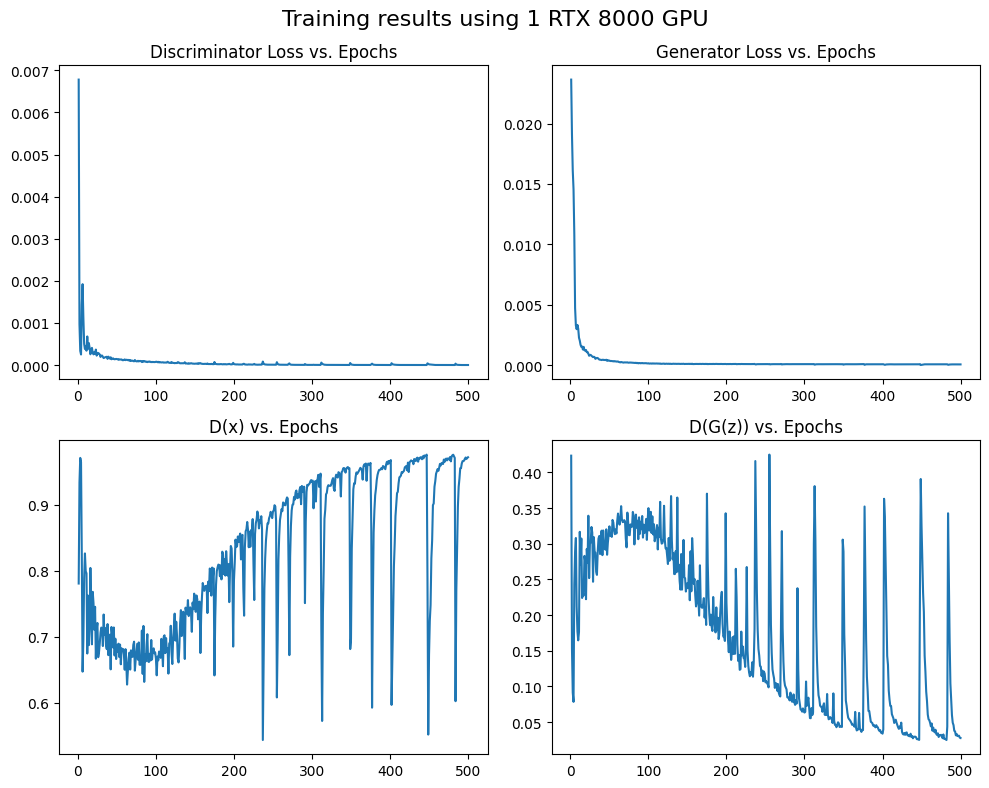
\includegraphics[scale = 0.3]{image/loss.png}
  \caption{Generator and Discriminator loss vs epoch graph for GAN network}\label{fig:loss}
%  \label{fig:fig2}
\end{figure}

IN Fig \ref{fig:loss} the loss function for two models have been decreased over time. 

-$D(x)$: This is the average output of the discriminator for real samples. In a typical GAN, the discriminator outputs a value between 0 and 1 for each sample, where 1 means the discriminator thinks the sample is completely real. So, $D(x)$ is the average of these outputs for the real samples in the current batch. If $D(x)$ is close to 1, it means the discriminator is correctly identifying real samples.

- $D(G(z))$: This is the average output of the discriminator for fake (generated) samples, before and after the generator update. The generator creates fake samples from a random input $z$, so $G(z)$ represents the fake samples. $D(G(z))$ is the average of the discriminator's outputs for these fake samples. The two numbers correspond to the average output before and after the generator is updated. If the first number is close to 0, it means the discriminator is correctly identifying fake samples before the generator update. If the second number is close to 1, it means the generator is doing a good job of fooling the discriminator after its update.

In your case, the discriminator loss is very low, which means the discriminator is doing a good job of identifying real and fake samples. The generator loss is also quite low, meaning the generator is also performing well. The $D(x)$ value is close to 1, meaning the discriminator is correctly identifying real samples, and the $D(G(z))$ value is relatively low, meaning the discriminator is also correctly identifying fake samples. However, the second $D(G(z))$ value is also relatively low, which suggests that the generator could be doing a better job of fooling the discriminator.
\begin{figure}[htbp]
\captionsetup[subfigure]{justification=centering}
  \centering
  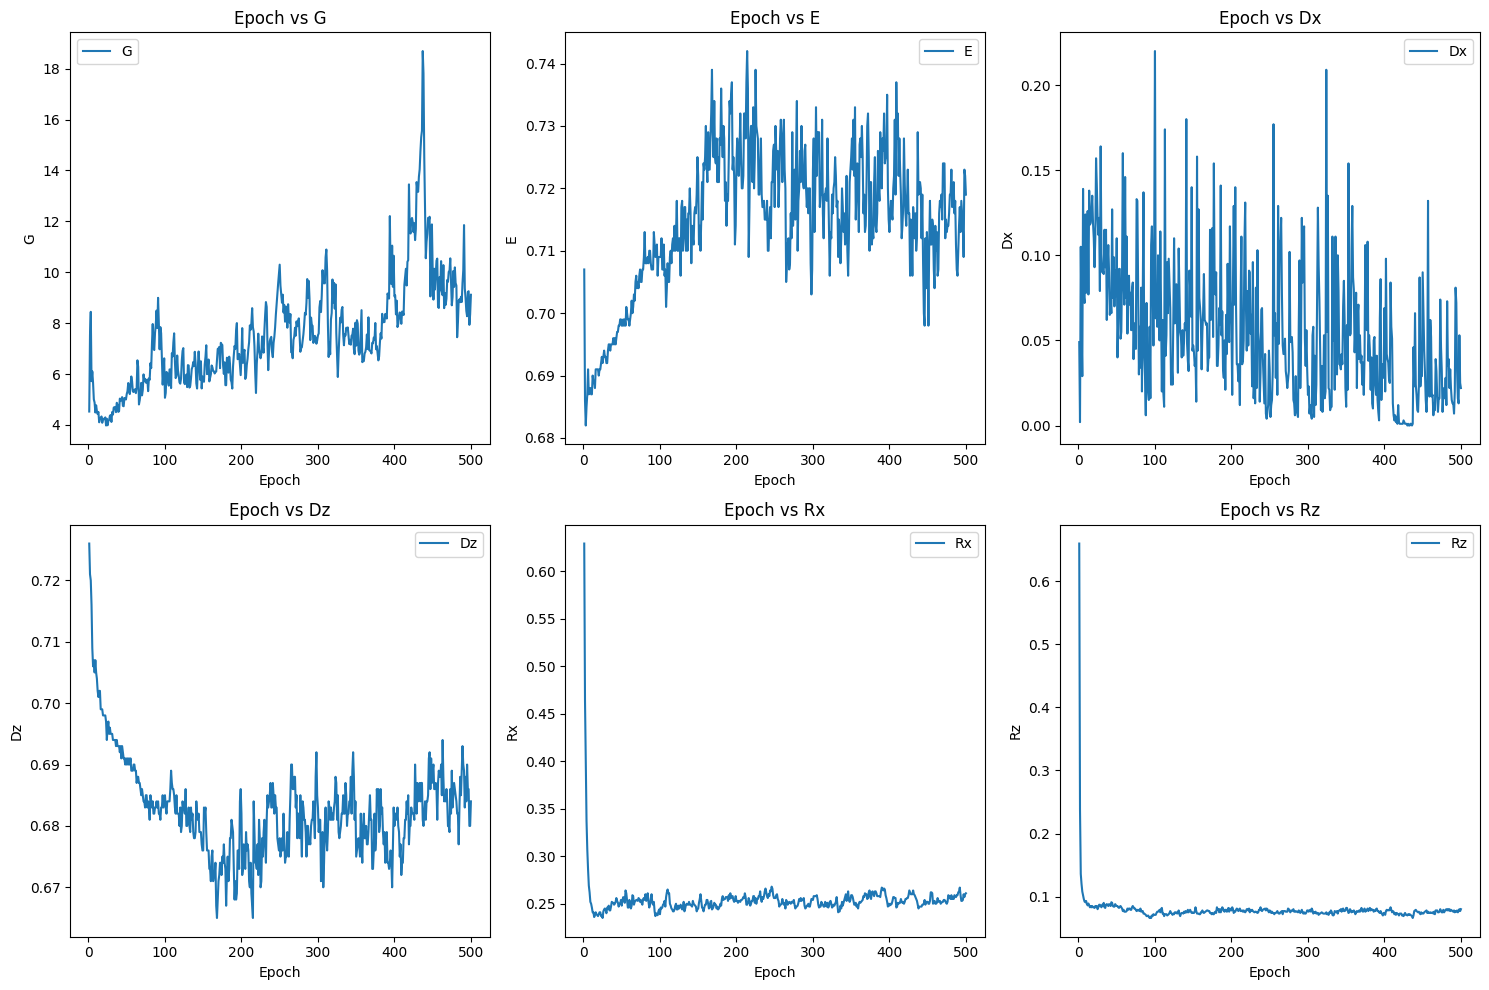
\includegraphics[scale = 0.2]{image/AEGAN loss.png}
  \caption{Hyper-parameters and loss vs epoch graph for AEGAN network}\label{fig:AEloss}
%  \label{fig:fig2}
\end{figure}

In the Fig \ref{fig:AEloss}, brife explanation of each parameters are as follow: 

- $G$: This is the generator's loss. The generator tries to minimize this value, which measures how well the generator is fooling the discriminator. 

- $E$: This is the encoder's loss. The encoder tries to minimize this value, which measures how well the encoder is able to map real images to the latent space.

- $Dx$: This is the discriminator's loss when evaluating real images. The discriminator tries to maximize this value, which measures how well the discriminator is able to classify real images as real.

- $Dz$: This is the discriminator's loss when evaluating generated images. The discriminator tries to maximize this value, which measures how well the discriminator is able to classify generated images as fake.

- $Rx$: This is the reconstruction loss for real images. The autoencoder tries to minimize this value, which measures how well the autoencoder is able to reconstruct real images.

- $Rz$: This is the reconstruction loss for generated images. The autoencoder tries to minimize this value, which measures how well the autoencoder is able to reconstruct generated images.

\section{Conclusion}

We conducted training for both the GAN and AEGAN models over a span of 500 epochs. However, we acknowledge that achieving even better quality results would require additional epochs, which is a time-consuming, computationally intensive, and expensive process. Nevertheless, the outcomes we obtained from the AEGAN model, as demonstrated by the provided Pokémon examples, exhibit enhanced details and clearer shapes after 500 epochs of training.

The AEGAN technique offers several improvements to typical GAN training, including training stabilization, mode-collapse prevention, and permitting the direct interpolation between real samples. The effectiveness of the technique is evident when comparing the results depicted in Figure \ref{fig:pok1} and \ref{fig:pok2}. 

However this model also has its own limitations. The primary limitation of the AEGAN technique is that it effectively doubles the size of the network, from two sub-networks to four, requiring more time and resources to train. 



% \begin{table}[h]
%     \centering
%     \caption{Train and test accuracy comparisons for models}
%     \label{tab:example}
%     \resizebox{0.95\columnwidth}{!}{
%     \begin{tabular}{|c|c|c|c|}
%         \hline
%         Models &Parameters & Train Accuracy & Test Accuracy \\
%         \hline
%         ResNetSmall & $78,042$ & $79.18\%$ & $79.40\%$\\
%         \hline 
%         ResNetMedium & $1,228,970$ & $91.06\%$ & $87.99\%$\\
%         \hline
%         ResNetLarge & $4,903,242$ & $94.16\%$ & $89.66\%$ \\
%         \hline
%     \end{tabular}
%     }
% \end{table}

\section{System Specification}
NYU HPC VM \\
CPU: 24 Virtualized Cores of Intel Xeon-Platinum 8286 \\
GPU: 4x Nvidia Quadro RTX 8000 \\
System Memory: 128 GB \\
Python Version: 3.8.6 \\
CUDA version: v11.8 \\
Torch Version: 2.0.0 \\

\section{Acknowledgment}
We would like to acknowledge the use of OpenAI's GPT-3.5 language model, commonly referred to as ChatGPT, for providing assistance with generating content for certain sections of this report.
\section{Literature Survey}
Generative Adversarial Networks (GANs) \cite{GAN} are a class of machine learning models that include a generator and a discriminator trained together to produce realistic data samples. This paper's contribution lies in utilizing GANs for generating new Pokémon spirits.

Autoencoding Generative Adversarial Networks (AEGANs) \cite{AEGAN} have proven effective in generating realistic images, and the quality of generated images can be further enhanced using a two-stage GAN architecture. By referencing this paper and its model, we improved the GAN model and achieved higher-quality results.

Adversarial Autoencoders\cite{encod} introduced a hybrid model that combines autoencoders and GANs, showcasing its effectiveness in generating realistic images of handwritten digits and faces. This paper provided insights on leveraging encoders and their combination with GANs.

To leverage the power of NYU HPC's multiple GPUs, we will employ PyTorch Distributed DataParallel and apply the knowledge gained to train models efficiently. 
\bibliography{aaai22}. \\
% \bibentry{c:25}.
%\nobibliography{aaai22}

\end{document}
